% 几何矢量
% 线性代数|几何矢量|代数矢量|单位矢量|标量|平行四边形法则|线性组合|线性相关|线性无关|基底|矢量空间|坐标

我们来回顾高中学的\textbf{几何矢量}, 本文中简称为“矢量”. 矢量是空间中的一些有长度有方向的箭头. 我们对它的位置不感兴趣, 所有长度和方向相同的矢量都视为同一矢量. 本书中矢量用正黑体表示, 如 $\bvec a$. 在手写时, 可以在字母上方加箭头表示, 如 $\overrightarrow{a}$. 特殊地, 如果一个矢量的长度等于 1, 那么它就是一个\textbf{单位矢量}, 本书中在矢量上面加上 “\^{}” 符号表示单位矢量, 如 $\uvec a$. 为了与矢量区分, 我们把单个的实数或复数称为\textbf{标量}.

\subsection{几何矢量}

\textbf{矢量(vector)}又被翻译为\textbf{向量}.这个概念最初来自直观的几何矢量.早在民国时期,学者们引入vector的概念时就将它译成了汉语.乌龙的是,由于当时的物理学家和数学家没有太多交集,双方相互独立地翻译了这个词:物理学家将它翻译为向量,而数学家翻译为矢量.90年代时,国家名词委员会商议确定一个统一的vector译名,但却无法轻易割舍两个译名中的任何一个,因为它们都非常信达雅地表明了vector的含义:向量即有方向的量,矢量即像箭矢一样的量.大概是出自物理学家和数学家的互相尊重,最后确定的方案是双方互换译名,从此物理学界称矢量,数学界称矢量.至今,台湾省物理学界依然将其译为向量\footnote{以下加粗部分为力学家朱照宣教授的回忆.\textbf{其实,在历史上,数学界曾把vector定名为“矢量”,而物理界曾把它定名为“向量”.后来,可能是为了尊重对方,却对换了一下,数学用向量,物理用矢量.在20世纪90年代初,国家名词委为此(vector)召开会议,想协调双方,由主任钱三强亲自主持.我曾戏称这是个“一字会”.当时的情况是,学科有分支,术语有派生,犹如家族有后裔.祖宗互相谦让,但子孙繁多,已无法协调.钱先生在会上没有说倾向于哪方面的话.矢量、向量的分歧,一直维持到今.力学这学科,和数学、物理同样有“亲”,力学中vector用什么? 当年我在“一字会”后还有情绪,埋怨钱先生作为领导“不表态”.过了好些年,才懂得这类事,最多只能因势利导,不能靠行政命令或专家拍板.事实上,台湾物理界至今用的是还“向量”.}   }.

本书中不区分两个译名的使用,在偏物理的话题上倾向于使用矢量,在偏数学或者抽象程度较高的话题上倾向于使用向量,希望读者注意.

\textbf{几何矢量}就是一种具有\textbf{长度}和\textbf{方向}的量,因此可以画成箭头来表示.生活中这样具有长度和方向的量十分常见:\textbf{速度}有大小有方向,因此可以表示为箭头,箭头的长度代表速度的大小;\textbf{加速度}也有大小,有方向;我从一个地方运动到另一个地方,那么从起点到终点可以画一根箭头,这箭头就是\textbf{位移矢量}.不止在生活中,一切领域里具有方向和大小概念的量都被称为几何矢量.不过,在数学中,向量的含义要比几何矢量更广泛,也就是说,几何矢量是数学家所研究的向量的一种,但不是唯一的一种.作为一个预热,在线性代数中,我们把这些最为直观的几何矢量构成的集合,称作“实数域上的赋范线性空间”.

特别地,长度为零的向量不作方向区分,称为\textbf{零向量}.零向量依然是向量,要注意和数字零进行区分.

几何矢量本身可以单独存在,而不需要借助任何坐标系或坐标来描述.事实上,随着坐标系的不同,一个矢量的坐标也往往不同.下面要介绍的许多概念(加法, 数乘, 线性组合, 线性无关等)都不需要任何坐标的概念,请试着摆脱具体的坐标来理解它们.

另外,对于几何矢量在高中数学以及几何学中的用途,张景中院士的《绕来绕去的向量法》一书的内容通俗易懂且干货充足,单墫的《向量与立体几何(数学奥林匹克命题人讲座)》也是一本实用的小册子,不过其符号的使用和主流稍有不同.感兴趣的读者可用这两本读物作参考.另外,数学界也借用物理中“质心”的概念,发展出了“质点几何学”分支,其本质仍然和向量几何一模一样,只不过换了个观点看问题;在上述张景中院士的书中提到了质点几何学,而网上也可以方便地搜到莫绍揆教授的《质点几何学》,但并不建议读者花太多精力学习,因为内容和向量几何完全重叠,只是对于部分几何问题的解答思路比向量几何更为易懂,实际意义不大\footnote{如果你好奇的话,只需要知道向量法中的\textbf{定比分点公式}就是连接质点几何和向量几何的桥梁,就可以把几何问题在这两个观点之间互相转化了.}.

\subsection{几何矢量的运算}

把所有几何矢量收集到一起,构成一个集合,本身没什么可以研究的.在集合\upref{Set}中我们说过,没有任何附加结构的集合中,元素叫什么都不重要,只有元素数量重要.为了让矢量集合有讨论的意义,我们引入了矢量的运算,这样,矢量集合就有了运算结构.

\subsubsection{矢量的加法}
第一个矢量运算,是矢量间的加法.两个矢量相加,结果是另一个矢量,其定义如下.

如\autoref{GVec_fig1},两个矢量相加, 既可以使用平行四边形法则, 也可以用三角形法则. 若有多个矢量连续相加, 可以分别把它们首尾相接, 结果就是由起点指向终点的矢量. 容易证明矢量的加法满足加法交换律 $\bvec A + \bvec B = \bvec B + \bvec A$, 结合律 $(\bvec A + \bvec B) + \bvec C = \bvec A + (\bvec B + \bvec C)$.
\begin{figure}[ht]
\centering
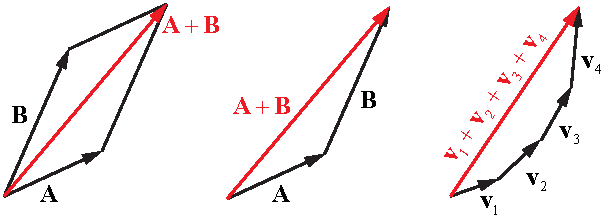
\includegraphics[width=10.5cm]{./figures/GVec_1.pdf}
\caption{矢量的加法} \label{GVec_fig1}
\end{figure}

\subsubsection{矢量的数乘\ 共线}
第二个矢量运算,是一个矢量和一个数字的乘积,得到一个矢量,称为数乘,我们用例子定义如下.

如\autoref{GVec_fig2}, 一个矢量与一个正实数相乘, 则方向不变, 把长度乘以这个实数. 若这个数是负数, 则把矢量取反方向再把长度乘以这个实数数的绝对值即可.若 $\lambda, \mu$ 表示实数, 容易证明分配律 $\lambda(\bvec A + \bvec B) = \lambda\bvec A + \lambda\bvec B$ 和 $(\lambda+\mu)\bvec A = \lambda\bvec A + \mu\bvec A$, 结合律 $\lambda(\mu\bvec A) = (\lambda\mu) \bvec A$.
\begin{figure}[ht]
\centering
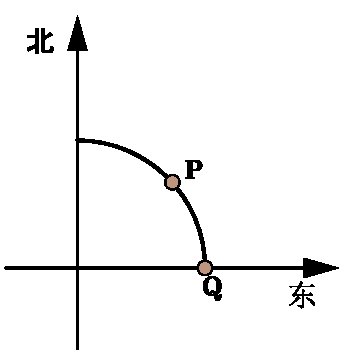
\includegraphics[width=6.5cm]{./figures/GVec_2.pdf}
\caption{矢量的数乘} \label{GVec_fig2}
\end{figure}

如果两个矢量的关系可以用 $\bvec A = \lambda\bvec B$ 表示, 那么它们就是\textbf{共线}的. 共线的充分必要条件\upref{SufCnd}是, 两矢量方向相同或相反.

\subsubsection{矢量的线性组合}
把有限个矢量 $\bvec v_i$ 分别与若干实数 $c_i$ 相乘再相加就得到了这些矢量的一个\textbf{线性组合}
\begin{equation}\label{GVec_eq1}
\sum_i^N c_i \bvec v_i = c_1\bvec v_1 + c_2\bvec v_2 +\dots +c_N \bvec v_N
\end{equation}

注意,若无特别说明,线性组合仅指\textbf{有限个}矢量的数乘和加法.

根据矢量加法和数乘的定义,容易得知任何有限个矢量的任何线性组合仍然是一个矢量.

\subsection{矢量空间}
矢量空间是一种矢量的集合,但不是任意的集合;一个矢量空间必须满足,在其中选择任意两个矢量,它们的线性组合仍然在这个空间中.进行归纳后易得,这个条件等价于“任意有限个矢量的线性组合仍然在这个空间中”.这个性质被称为矢量线性组合的\textbf{封闭性}.

矢量的线性组合,使得我们有可能用少量矢量来表示更多的矢量.给定若干矢量构成的集合$S=\{\bvec{v_\alpha}\}$,这个集合可以是无穷集合,那么从$S$中任意地选择有限个矢量进行线性组合,所得到的集合$\{\sum_i^N c_i\bvec{v_i}|N\in\mathbb{Z}, c_i\in\mathbb{R}, \bvec{v}_i\}$称为$S$所\textbf{张成(span)的空间},记为$<S>$或者$<\{v_\alpha\}>$.由于$v_\alpha$的线性组合的线性组合还是$v_\alpha$的线性组合,这个定义使得$<S>$必然是一个矢量空间.

\subsubsection{线性相关性}

如果存在至少一组不全为零系数 $c_i$ 使几个矢量的线性组合等于零, 这些矢量就被称为\textbf{线性相关}的
\begin{equation}\label{GVec_eq2}
\sum_i^N c_i \bvec v_i = \bvec 0
\end{equation}
这是因为对于任何一个不为零的项 $j$, 矢量 $\bvec v_j$ 都可以表示为其他矢量的线性组合. 只需把上式除以 $c_j$ 即可
\begin{equation}\label{GVec_eq3}
\bvec v_j = \sum_{i \ne j}\frac{c_i}{c_j} \bvec v_i
\end{equation}
如果不存在这样的系数, 这些矢量就是\textbf{线性无关}的. 

如果一个矢量集合中的矢量是线性相关的,那么这个集合被称为一个\textbf{线性相关组};反之,若线性无关,则称为一个\textbf{线性无关组}.

如果一组矢量之间线性相关,那么至少有一个矢量是“冗余”的,也就是说,它可以被其它矢量的线性组合表示出来.这样一来,对于线性相关的矢量组,如果用它们的线性组合来表示其它矢量,那么表示方式都不是唯一的.线性无关的矢量组,最重要的性质就是它们的线性组合表达式是唯一的,由此引入了基底、坐标等概念.

\subsection{基底\ 矢量空间\ 坐标}
沿一条直线的所有矢量都是共线的, 所以在一条直线上最多不超过一个矢量线性无关, 所有这些共线的矢量以及它们的加法和数乘运算组成一个\textbf{一维矢量空间}\footnote{注意这里并没不打算给出矢量空间的一般定义, 只是说 “是一个矢量空间”. 一般定义见 “矢量空间\upref{LSpace}”}. 一个平面上的所有矢量以及它们的加法和数乘运算, 组成一个\textbf{二维矢量空间}, 二维矢量空间中最多只能找到两个线性无关的矢量. \textbf{三维矢量空间}同理.一般地,$N$维矢量空间中的任意线性无关组最多只包含$N$个矢量.

$N$ 维空间中的任意一组线性无关的 $N$ 个矢量 $\bvec \beta_1\dots \bvec \beta_N$ 可以作为一组\textbf{基底(basis)}, 记为 $\{\bvec \beta_i\}$,简称\textbf{基}. 基是有序的, 即使是同一组矢量,如果顺序不同,也要视为不同的基. 

如果在这组基底中加入该空间中任意一个矢量 $\bvec v$, 这组 $N+1$ 个矢量必定线性相关(否则空间就是 $N+1$ 维的).

由于线性无关组所能表示的矢量,都只有唯一的表示;而添加一个矢量以后上述线性无关组就变成线性相关的了,意味着该空间中任何矢量都可以被这个线性无关组所表示,因此该空间中的一切矢量都可以被这个$N$元线性无关组\textbf{唯一地}表示.$\bvec v$ 可用 $\{\bvec \beta_i\}$ 的线性组合表示. 对于该空间中任意矢量 $\bvec v$,存在唯一一组系数$\{x_i\}_{i=1}^N$,使得
\begin{equation}\label{GVec_eq5}
\bvec v = \sum_{i=1}^N x_i \bvec \beta_i
\end{equation}
那么我们称$(x1, x2, \cdots, x_N)$是矢量$\bvec v$在\textbf{这个基}下的\textbf{坐标(coordinate)}.

显然,基底不同时,同一个矢量的坐标也不同,因此坐标\textbf{不能}简单地等同于矢量本身.只有在讨论中固定了基的选择时,才可以把坐标和矢量本身等同.

\begin{exercise}{计算坐标}
以上所说的坐标不一定是直角坐标系的坐标. 例如平面上两个基底 $\bvec \beta_1$ 与 $\bvec \beta_2$ 的长度分别为 1 和 2. 夹角为 $\pi/3$, 矢量 $\bvec v$ 恰好落在两个基底的角平分线上, 长度为 3. 求 $\bvec v$ 的坐标.答案:$1/\sqrt 3$, $1/(2\sqrt 3)$.
\end{exercise}

我们可以用反证法证明坐标的唯一性. 假设有两组不全相同的系数都可以使\autoref{GVec_eq5} 成立, 分别记为 $x_i$ 和 $y_i$. 那么分别代入上式再把两式相减得到
\begin{equation}
\sum_{i=1}^N (x_i-y_i) \bvec \beta_i = \bvec 0
\end{equation}
由于 $(x_i-y_i)$ 不全为零, 得到基底 $\{\bvec \beta_i\}$ 线性相关, 而这是不可能的.证毕.

\subsection{坐标的运算}
我们常常把一个矢量的坐标写成一个\textbf{代数矢量}, 如
\begin{equation}\label{GVec_eq7}
\bvec v = \pmat{x\\y\\z}_{\{\bvec\beta_i\}}
\end{equation}
在列矢量的右下角声明基底是较为严谨的做法, 但为了书写简洁, 在不至于混淆的情况下我们可以将其省略. 另外在正文中, 为了节约空间, 我们将\autoref{GVec_eq7} 记为 $\bvec v = (x, y, z)_{\{\bvec\beta_i\}}\Tr$(见“矩阵\upref{Mat}” \autoref{Mat_eq2} ),其中$\Tr$表示矩阵的转置.同样, 我们时常省略 $\{\bvec\beta_i\}$.

当我们说两个矢量\textbf{相等}时, 意味着同一基底下两矢量的坐标全都相等. 若已知两矢量在不同基底下的列矢量, 则需要先将它们变换到同一基底下再判断是否相等.

以上介绍的加法和数乘都有对应的坐标运算. 由\autoref{GVec_eq5} 及矢量加法和数乘的交换律和结合律得
\begin{equation}\label{GVec_eq8}
\bvec v_1 + \bvec v_2 = \pmat{x_1\\y_1\\z_1}_{\{\bvec\beta_i\}} + \pmat{x_2\\y_2\\z_2}_{\{\bvec\beta_i\}} = \pmat{x_1 + x_2\\y_1 + y_2\\z_1 + z_2}_{\{\bvec\beta_i\}}
\end{equation}
\begin{equation}\label{GVec_eq9}
\lambda \bvec v = \lambda\pmat{x\\y\\z}_{\{\bvec\beta_i\}} = \pmat{\lambda x\\\lambda y\\\lambda z}_{\{\bvec\beta_i\}}
\end{equation}

要特别注意的是, 当定义了多组基底时, 只有基底相同的两个列矢量按照\autoref{GVec_eq8} 相加才有意义.
